Das Ziel des Algorithmus zur Tassenerkennung ist es eine möglichst genaue quaderförmige Bounding Box für die Tasse zu errechnen. Der Algorithmus gliedert sich in folgende grobe Schritte:
\begin{itemize}
\item Detektion der Tasse in den Bilddaten
\item Segmentierung der Tasse aus der Punktwolke
\item Berechnung der Tassenorientierung.
\end{itemize}
Die einzelnen Schritte sollen in den nächsten Abschnitten detailliert beschrieben werden.
\paragraph{Detektion der Tasse in den Bilddaten}
Die Detektion der Tasse basiert auf der Klassifikation von Bildsegmenten mittels einer Support Vector Machine (SVM). Hierfür wird im Rahmen eines Sliding Window Ansatzes das ganze Bild durchlaufen und an jeder Stelle ein quadratisches Bildsegment extrahiert. Jedes dieser Bildsegmente soll im nächsten Schritt nun klassifiziert werden, wobei es sich hier um ein binäres Klassifikationsproblem (\glqq Tasse\grqq/\glqq Keine Tasse \grqq) handelt. Die Klassifikation jedes Segments erfolgt hierbei anhand zuvor extrahierter Histogram of Oriented Gradient (HOG) Features. Als Resultat gibt liefert die SVM eine Liste an Tupeln, welche die Wahrscheinlichkeiten der Klassenzugehörigkeiten eines jeden Segments enthalten. Die zuvor beschriebene Klassifikation wird hierbei in 8 Threads ausgeführt, was die benötigte Zeit in etwa halbiert. Für die Weiterverarbeitung werden nun die Bounding Boxen ausgewählt, welche gemäß der Klassifikation mit einer Wahrscheinlichkeit von mehr als 0.9 zur Klasse Tasse gehören. Zudem werden in diesem Schritt auch noch nah zusammenliegende Boundingboxen, welche vermutlich zum selben Objekt gehören, durch das Clustering ihrer Zentren mittels DBSCAN zusammengefasst.

\paragraph{Segmentierung der Tasse aus der Punktwolke}
Nachdem die Tasse in den Bilddaten erkannt wurde sollen nun die zugehörigen Punkte aus der Punkwolke segmentiert werden. Bevor die eigentlich Segmentierung durchgeführt wird, werden aber noch die zuvor berechneten Bounding Boxen mithilfe von Daten aus der Punktwolke auf Plausibilität überprüft. Hierbei wird überprüft, ob der Mittelwert der z-Koordinate der zur Bounding Box gehörenden Punkte weniger als 10cm von der Tischhöhe abweicht. So können beispielsweise zum Roboterarm gehörige Fehlerkennungen frühzeitig ausgeschlossen werden. Anschließend beginnt die eigentliche Segmentierung. Hierfür werden die Mittelwerte aller Koordinatenachsen des die Tasse enthaltenden Segments berechnet. Anschließend wird ein Bereich um die errechneten Koordinaten-Mittelwerte aus der Punktwolke herausgeschnitten und die Tischplatte aus der Punkwolke entfernt. Das herausgeschnittene Segment der Punktwolke enthält nun zwar schon die Tasse, ggf. sind aber noch einzelne andere Punkte enthalten. Um diese von der Tasse zu trennen wird wiederum das DCSCAN Clustering Verfahren angewandt und der größte gefundene Cluster als Tasse ausgewählt (siehe Abbildung \ref{fig:cup_segmentation}).

\paragraph{Berechnung der Tassenorientierung}
Aus dem vorhergehenden Schritt erhalten wir die Punkte der von der Kinect gelieferten Punktwolke, die zur Tasse gehören. Aus diesen soll nun die Orientierung des Tassenhenkels bestimmt werden. Unser Algorithmus stützt sich hier auf die Annahme, dass die zum Henkel gehörenden Punkte in einem deutlich weniger dicht besetzten Gebiet der Punktwolke liegen als die restlichen zur Tasse gehörigen Punkte. Um dies auszunutzen wenden wir den sogenannten Local Outlier Factor (LOF) Algorithmus an, welcher häufig zur Ausreißer Detektion verwendet wird indem er  die Dichte eines Punktes mit der seiner Nachbarn vergleicht. Die vom Algorithmus zurückgelieferten Ausreißer, welche eine geringere Dichte aufweisen als ihre Nachbarn betrachten wir im folgenden als zum Henkel gehörende Punkte (siehe Abbildung \ref{fig:orientation_detection}). Um aus ihnen die Orientierung des Henkels zu bestimmen genügt es, das Zentrum der Tassenpunktwolke mit dem Durschnittswert der zum Henkel gehörigen Punkte zu verbinden und den Winkel zwischen der y-Achse und dem so berechneten Vektor zu bestimmen.

\begin{figure}
    \centering
    \begin{minipage}{0.45\textwidth}
        \centering
        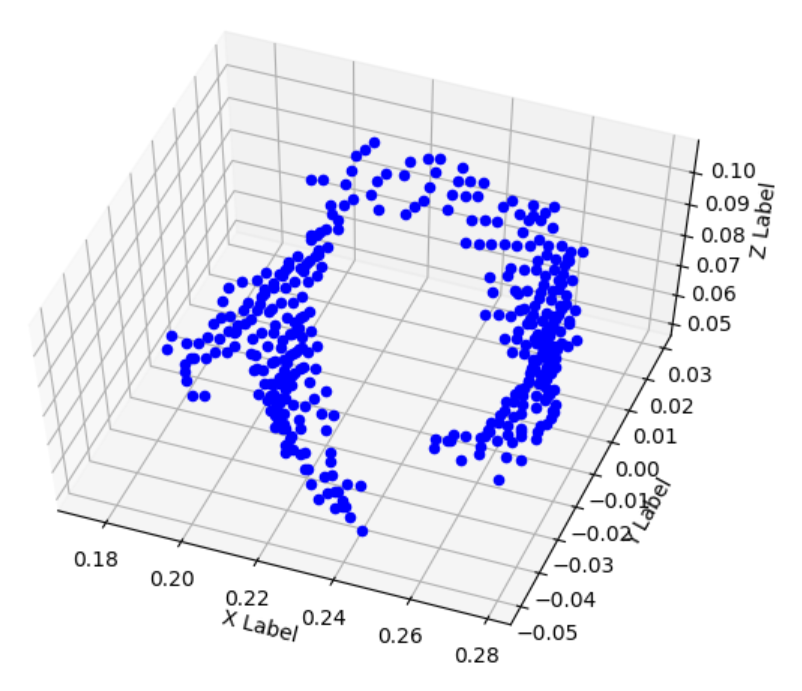
\includegraphics[width=0.9\textwidth]{images/cup_3d.png} % first figure itself
        \caption{Segmentierung der Tasse aus der Punktwolke \label{fig:cup_segmentation}}
    \end{minipage}\hfill
    \begin{minipage}{0.45\textwidth}
        \centering
        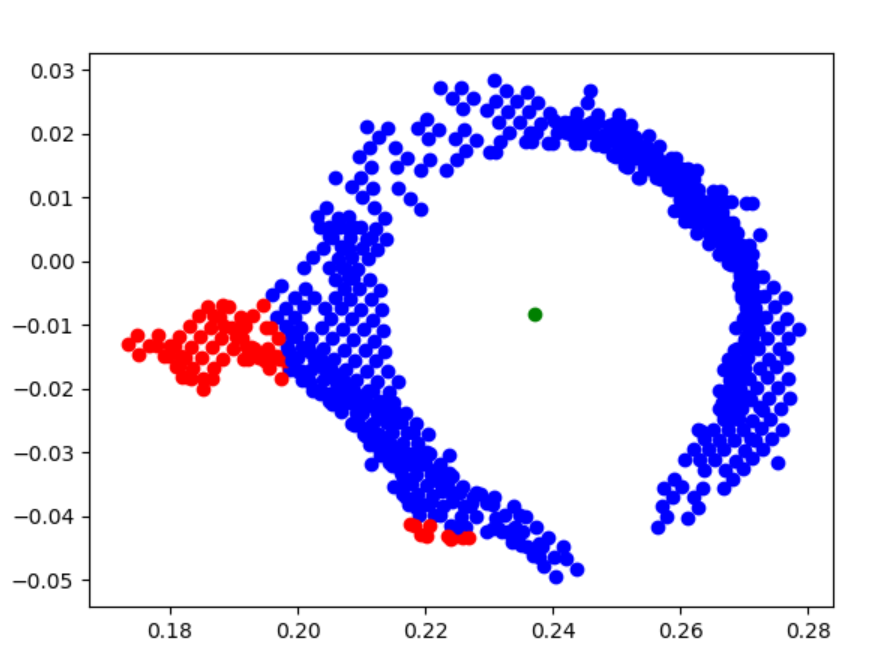
\includegraphics[width=0.9\textwidth]{images/cup_handle.png} % second figure itself
        \caption{Orientierungserkennung mittels LOF \label{fig:orientation_detection}}
    \end{minipage}
\end{figure}